\section{Đề số 1}
\graphicspath{{./img/}}

\begin{bt}
    \hfill
    \begin{enumerate}[a.]
        \item Thực hiện phép tính: $\frac{0,375-0,3+\frac{3}{11}+\frac{3}{12}}{-0,265+0,5-\frac{5}{11}-\frac{5}{12}}+\frac{1,5+1-0,75}{2,5+\frac{5}{3}-1,25}$
        \item So sánh: $\sqrt{50}+\sqrt{26}+1 \quad$ và $\sqrt{168}$.
    \end{enumerate}
\loigiai{
    \begin{enumerate}[a.]
        \item Ta có: $\mathrm{A}=\frac{\frac{3}{8}-\frac{3}{10}+\frac{3}{11}+\frac{3}{12}}{-\frac{53}{100}+\frac{5}{10}-\frac{5}{11}-\frac{5}{12}}+\frac{\frac{3}{2}+\frac{3}{3}-\frac{3}{4}}{\frac{5}{2}+\frac{5}{3}-\frac{5}{4}}$\\
        $\begin{aligned} & =\frac{3\left(\frac{1}{8}-\frac{1}{10}+\frac{1}{11}+\frac{1}{12}\right)}{\frac{-53}{100}-5\left(-\frac{1}{10}+\frac{1}{11}+\frac{1}{12}\right)}+\frac{3\left(\frac{1}{2}+\frac{1}{3}-\frac{1}{4}\right)}{5\left(\frac{1}{2}+\frac{1}{3}-\frac{1}{4}\right)}=\frac{3\left(\frac{165-132+120+110}{1320}\right)}{\frac{-53}{100}-5\left(\frac{-66+60+55}{660}\right)}+\frac{3}{5} \\ & =\frac{3 \cdot \frac{263}{1320}}{\frac{-53}{100}-5 \cdot \frac{49}{660}}+\frac{3}{5}=\frac{3 \cdot \frac{263}{1320}}{\frac{-1749-1225}{3300}}+\frac{3}{5}=\frac{3945}{-5948}+\frac{3}{5}=\frac{-1881}{29740}\end{aligned}$
        \item Ta có: $\sqrt{50}>\sqrt{49}=4 ; \sqrt{26}>\sqrt{25}=5$\\
        Vậy: $\sqrt{50}+\sqrt{26}+1>7+5+1=13=\sqrt{169}>\sqrt{168}$
    \end{enumerate}
} 
\end{bt}

\begin{bt}
    \hfill
    \begin{enumerate}[a.]
        \item Tìm $x$ biết: $|x-2|+|3-2 x|=2 x+1$
        \item Tìm $x ; y \in Z$ biết: $x y+2 x-y=5$
        \item Tìm x; y; z biết: $2 x=3 y$ ; $4 y=5 z$ và $4 x-3 y+5 z=7$
    \end{enumerate}
\loigiai{
    \begin{enumerate}[a.]
        \item Nếu $x>2$ ta có: $x-2+2 x-3=2 x+1 \Leftrightarrow x=6$\\
        Nếu $\frac{3}{2} \leq x \leq 2$ ta có: $2-\mathrm{x}+2 \mathrm{x}-3=2 \mathrm{x}+1 \Leftrightarrow \mathrm{x}=-2$ loại\\
        Nếu $x<\frac{3}{2}$ ta có: $2-x+3-2 x=2 x+1 \Leftrightarrow x=\frac{4}{5}$\\
        Vậy: $x=6 ; x=\frac{4}{5}$
        \item Ta có: $x y+2 x-y=5 \Leftrightarrow x(y+2)-(y+2)=3$
        $\\
        \Leftrightarrow(y+2)(x-1)=3 \cdot 1=1 \cdot 3=(-1) \cdot(-3)=(-3) \cdot(-1)
        $\\
        $$
        \begin{tabular}{|c|c|c|c|c|}
        \hline $\mathrm{y}+2$ & 3 & 1 & $-1$ & $-3$ \\
        \hline $\mathrm{x}-1$ & 1 & 3 & $-3$ & $-1$ \\
        \hline $\mathrm{x}$ & 2 & 4 & $-2$ & 0 \\
        \hline $\mathrm{y}$ & 1 & $-1$ & $-3$ & $-5$ \\
        \hline
        \end{tabular}
$$
        \item Từ: $2 x=3 y ; 4 y=5 z \Rightarrow 8 x=12 y=15 z$
        $\\
        \begin{aligned}
        & \Rightarrow \frac{x}{\frac{1}{8}}=\frac{y}{\frac{1}{12}}=\frac{z}{\frac{1}{15}}=\frac{4 x}{\frac{1}{2}}=\frac{3 y}{\frac{1}{4}}=\frac{5 z}{\frac{1}{3}}=\frac{4 x-3 y+5 z}{\frac{1}{2}=\frac{1}{4}+\frac{1}{3}}=\frac{7}{\frac{7}{12}}=12 \\
        & \Rightarrow \mathrm{x}=12 \cdot \frac{1}{8}=\frac{3}{2} ; \mathrm{y}=12 \cdot \frac{1}{12}=1 ; \mathrm{z}=12 \cdot \frac{1}{15}=\frac{4}{5}
        \end{aligned}
        $
    \end{enumerate}
} 
\end{bt}

\begin{bt}
    \hfill
    \begin{enumerate}[a.]
        \item Tìm đa thức bậc hai biết $f(x)-f(x-1)=x$.
        
        Từ đó áp dụng tính tổng $\mathrm{S}=1+2+3+\ldots+\mathrm{n}$.
        \item Cho $\frac{2 b z-3 c y}{a}=\frac{3 c x-a z}{2 b}=\frac{a y-2 b x}{3 c}$
        
        Chứng minh: $\frac{x}{a}=\frac{y}{2 b}=\frac{z}{3 c}$.
    \end{enumerate}
\loigiai{
    \begin{enumerate}[a.]
        \item  Đa thức bậc hai cần tìm có dạng: $f(x)=a x^2+b x+c \quad(\mathrm{a} \neq 0)$.\\
        Ta có : $f(x-1)=a(x-1)^2+b(x-1)+c$.\\
        $
        f(x)-f(x-1)=2 a x-a+b=x \Rightarrow\left\{\begin{array} { l } 
        { 2 a = 1 } \\
        { b - a = 0 }
        \end{array} \Rightarrow \left\{\begin{array}{l}
        a=\frac{1}{2} \\
        b=\frac{1}{2}
        \end{array}\right.\right.
        $\\
        Vậy đa thức cần tìm là: $f(x)=\frac{1}{2} x^2+\frac{1}{2} x+c$ (c là hằng số tùy ý).\\
        Áp dụng:
        $$
        \begin{aligned}
        & +\text { Với } x=1 \text { ta có }: 1=f(1)-f(0) \\
        & +\text { Với } x=2 \text { ta có }: 1=f(2)-f(1)
        \end{aligned}
        $$
        $$
        \begin{aligned}
        & +\text { Với } \mathrm{x}=\mathrm{n} \text { ta có }: n=f(n)-f(n-1) \\
        & \Rightarrow \mathrm{S}=1+2+3+\ldots+\mathrm{n}=f(n)-f(0)=\frac{n^2}{2}+\frac{n}{2}+c-c=\frac{n(n+1)}{2}
        \end{aligned}
        $$
        \item Ta có: $\frac{2 b z-3 c y}{a}=\frac{3 c x-a z}{2 b}=\frac{a y-2 b x}{3 c} \\
        \Leftrightarrow \frac{2 a b z-3 a c y}{a^2}=\frac{6 b c x-2 a b z}{4 b^2}=\frac{3 a c y-6 b c x}{9 c^2}\\ 
        =\frac{2 a b z-3 a c y+6 b c x-2 a b z+3 a c y-6 b c x}{a^2+4 b^2+9 c^2}=0 \\
        \Rightarrow 2 \mathrm{bz}-3 \mathrm{cy}=0 \Rightarrow \frac{z}{3 c}=\frac{y}{2 b}(1) \\
        \Rightarrow 3 c x-a z=0 \Rightarrow \frac{x}{a}=\frac{z}{3 c}(2) ;\\ 
        \text { Từ (1) và (2) suy ra: } \frac{x}{a}=\frac{y}{2 b}=\frac{z}{3 c}$
    \end{enumerate}
}
\end{bt}

\begin{bt}
    \hfill
    Cho tam giác $\mathrm{ABC}\left(B A C<90^{\circ}\right)$, đường cao $\mathrm{AH}$. Gọi $\mathrm{E} ; \mathrm{F}$ lần lượt là điểm đối xứng của $\mathrm{H}$ qua $\mathrm{AB} ; \mathrm{AC}$, đường thẳng $\mathrm{EF}$ cắt $\mathrm{AB} ; \mathrm{AC}$ lần lượt tại $\mathrm{M}$ và $\mathrm{N}$. Chứng minh rằng:
    \begin{enumerate}[a.]
    \item $\mathrm{AE}=\mathrm{AF}$;
    \item HA là phân giác của $M H N$;
    \item $\mathrm{CM} / / \mathrm{EH} ; \mathrm{BN} / / \mathrm{FH}$.
    \end{enumerate}
\loigiai{
    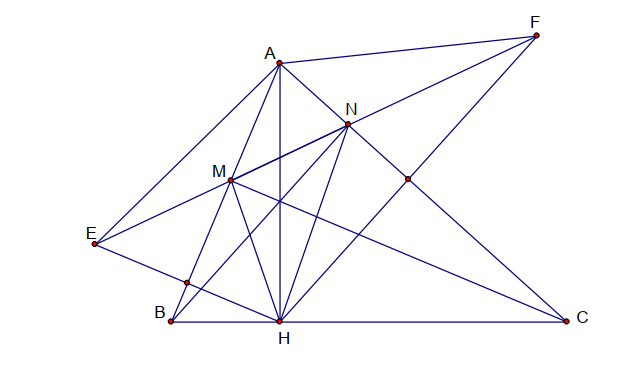
\includegraphics[width=0.7\textwidth]{1-4-lg.png}
    \begin{enumerate}
        \item Vì $\mathrm{AB}$ là trung trực của $\mathrm{EH}$ nên ta có: $\mathrm{AE}=\mathrm{AH}$ (1) \\
        Vì $\mathrm{AC}$ là trung trực của $\mathrm{HF}$ nên ta có: $\mathrm{AH}=\mathrm{AF}$ (2) \\
        Từ (1) và $(2)$ suy ra: $\mathrm{AE}=\mathrm{AF}$
        \item Vì $\mathrm{M} \in \mathrm{AB}$ nên $\mathrm{MB}$ là phân giác $E M H \Rightarrow \mathrm{MB}$ là phân giác ngoài góc $\mathrm{M}$ của tam giác $\mathrm{MNH}$ \\
        Vì $\mathrm{~N} \in \mathrm{AC}$ nên $\mathrm{NC}$ là phân giác $F N H \Rightarrow \mathrm{NC}$ là phân giác ngoài góc $\mathrm{N}$ của tam giác MNH \\
        Do $\mathrm{MB}$; $\mathrm{NC}$ cắt nhau tại $\mathrm{A}$ nên $\mathrm{HA}$ là phân giác trong góc $\mathrm{H}$ của tam giác $\mathrm{HMN}$ hay HA là phân giác của $M H N$.
        \item Ta có $\mathrm{AH} \perp \mathrm{BC}$ (gt) mà $\mathrm{HM}$ là phân giác $M H N \Rightarrow \mathrm{HB}$ là phân giác ngoài góc $\mathrm{H}$ của tam giác $\mathrm{HMN}$ \\
        $M B$ là phân giác ngoài góc $M$ của tam giác $\mathrm{HMN}(\mathrm{cmt}) \Rightarrow \mathrm{NB}$ là phân giác trong góc $\mathrm{N}$ của tam giác $\mathrm{HMN}$ \\
        $\Rightarrow \mathrm{BN} \perp \mathrm{AC}$ ( Hai đường phân giác của hai góc kề bù thì vuông góc với nhau). $\Rightarrow$ $\mathrm{BN} / / \mathrm{HF}$ ( cùng vuông góc với $\mathrm{AC}$ )
        Chứng minh tương tự ta có: $\mathrm{EH} / / \mathrm{CM}$
    \end{enumerate}
}
\end{bt}